\section{The Takamaka Language for Smart Contracts}\label{sec:takamaka}

This section gives a short introduction to the Takamaka subset of
Java that this paper uses for writing smart contracts.
This language has been introduced in~\cite{Spoto19}. A full tutorial
is available online, as part of the documentation of the Hotmoka
blockchain that runs smart contracts written
in Takamaka~\cite{hotmoka_repository}. This section introduces only
the essential notions that are needed to understand the subsequent sections.
The hierarchy of the classes described in this section is in Fig.~\ref{fig:hierarchy-entities}.
In the following, a simplified presentation of the code of some
of such classes will be reported. The full code is in the Github repository of Hotmoka~\cite{hotmoka_repository}.

\begin{figure*}[t]
  \begin{center}
    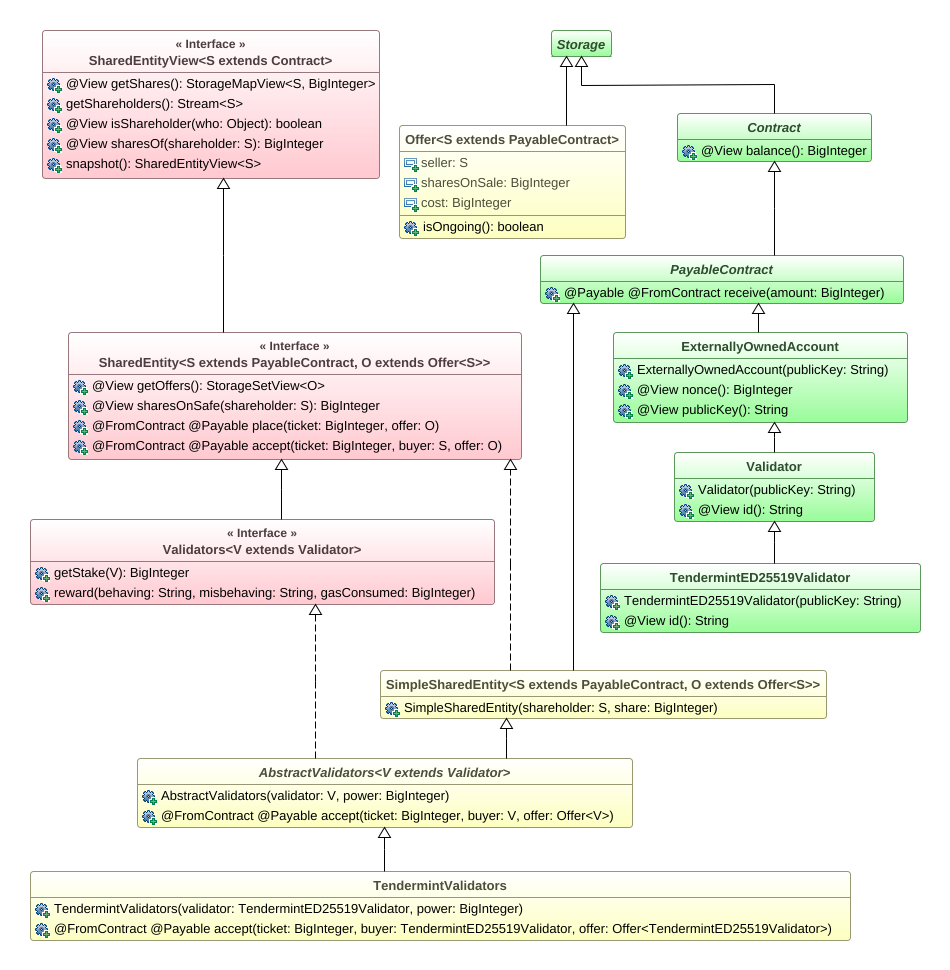
\includegraphics[width=12.2cm]{entities-hierarchy.png}
  \end{center}
  \caption{The hierarchy of Takamaka classes that implement accounts, shared entities and validators. Their source code can be found inside the Java project \textsf{\url{https://github.com/Hotmoka/hotmoka/tree/master/io-takamaka-code}}.}\label{fig:hierarchy-entities}
\end{figure*}

Takamaka implements objects persisted in blockchain as subclasses of the class
\<io.takamaka.code.lang.Storage>.
This is the main difference with other attempts at using Java for writing smart contracts:
the programmer does not code the serialization and deserialization of objects into
a \emph{keeper} or a key/value map, but simply extends \<Storage> and objects get
persisted automatically \emph{out of magic}. In this sense, Takamaka follows the approach of
Solidity, but using Java.

The \<io.takamaka.code.lang.Contract> class implements objects that can be
persisted in blockchain \emph{and} have a balance. Therefore, they can receive and provide payments.
Their balance is available through a \<balance> method. This is a \<@View> method, meaning
that it can be called without paying gas (the measure of execution cost), since such methods
cannot have side-effects and consequently do not modify the storage of the blockchain.
Payments can be received only through methods annotated as \<@Payable>.
The \<Contract> superclass has no such methods, but subclasses may have.
For instance, its \<io.takamaka.code.lang.PayableContract> subclass has
a method \<receive> to receive payments from its caller. Many methods (inclusing all
\<@Payable> methods) need to identify their caller. This is done by adding the
\<@FromContract> annotation, that guarantees that the caller is a contract, available
inside the method as \<caller()>.

Method calls started from outside the blockchain (for instance, from a client such as a wallet
or from a web application), must specify an already existing \<ExternallyOwnedAccount>
as caller. This account will pay for the gas of the execution. The blockchain will accept
the call only if is signed with the private key that matches the public key provided to
the constructor of the account when it was created. Method \<publicKey> allows one to
recover that public key and method \<nonce> allows one to get a progressive identifier that
can be used to distinguish successive calls with the same account, to force their order
of execution and to avoid replaying.
All that is very similar to Solidity, except for the fact that externally owned accounts
are actual Java objects inside the blockchain, not just an abstraction of a public key. An exemplification of a call made to a \<PayableContract> is reported in Fig.\,\ref{figure.takamaka_payable_contract}

\begin{figure}[ht]
\centering
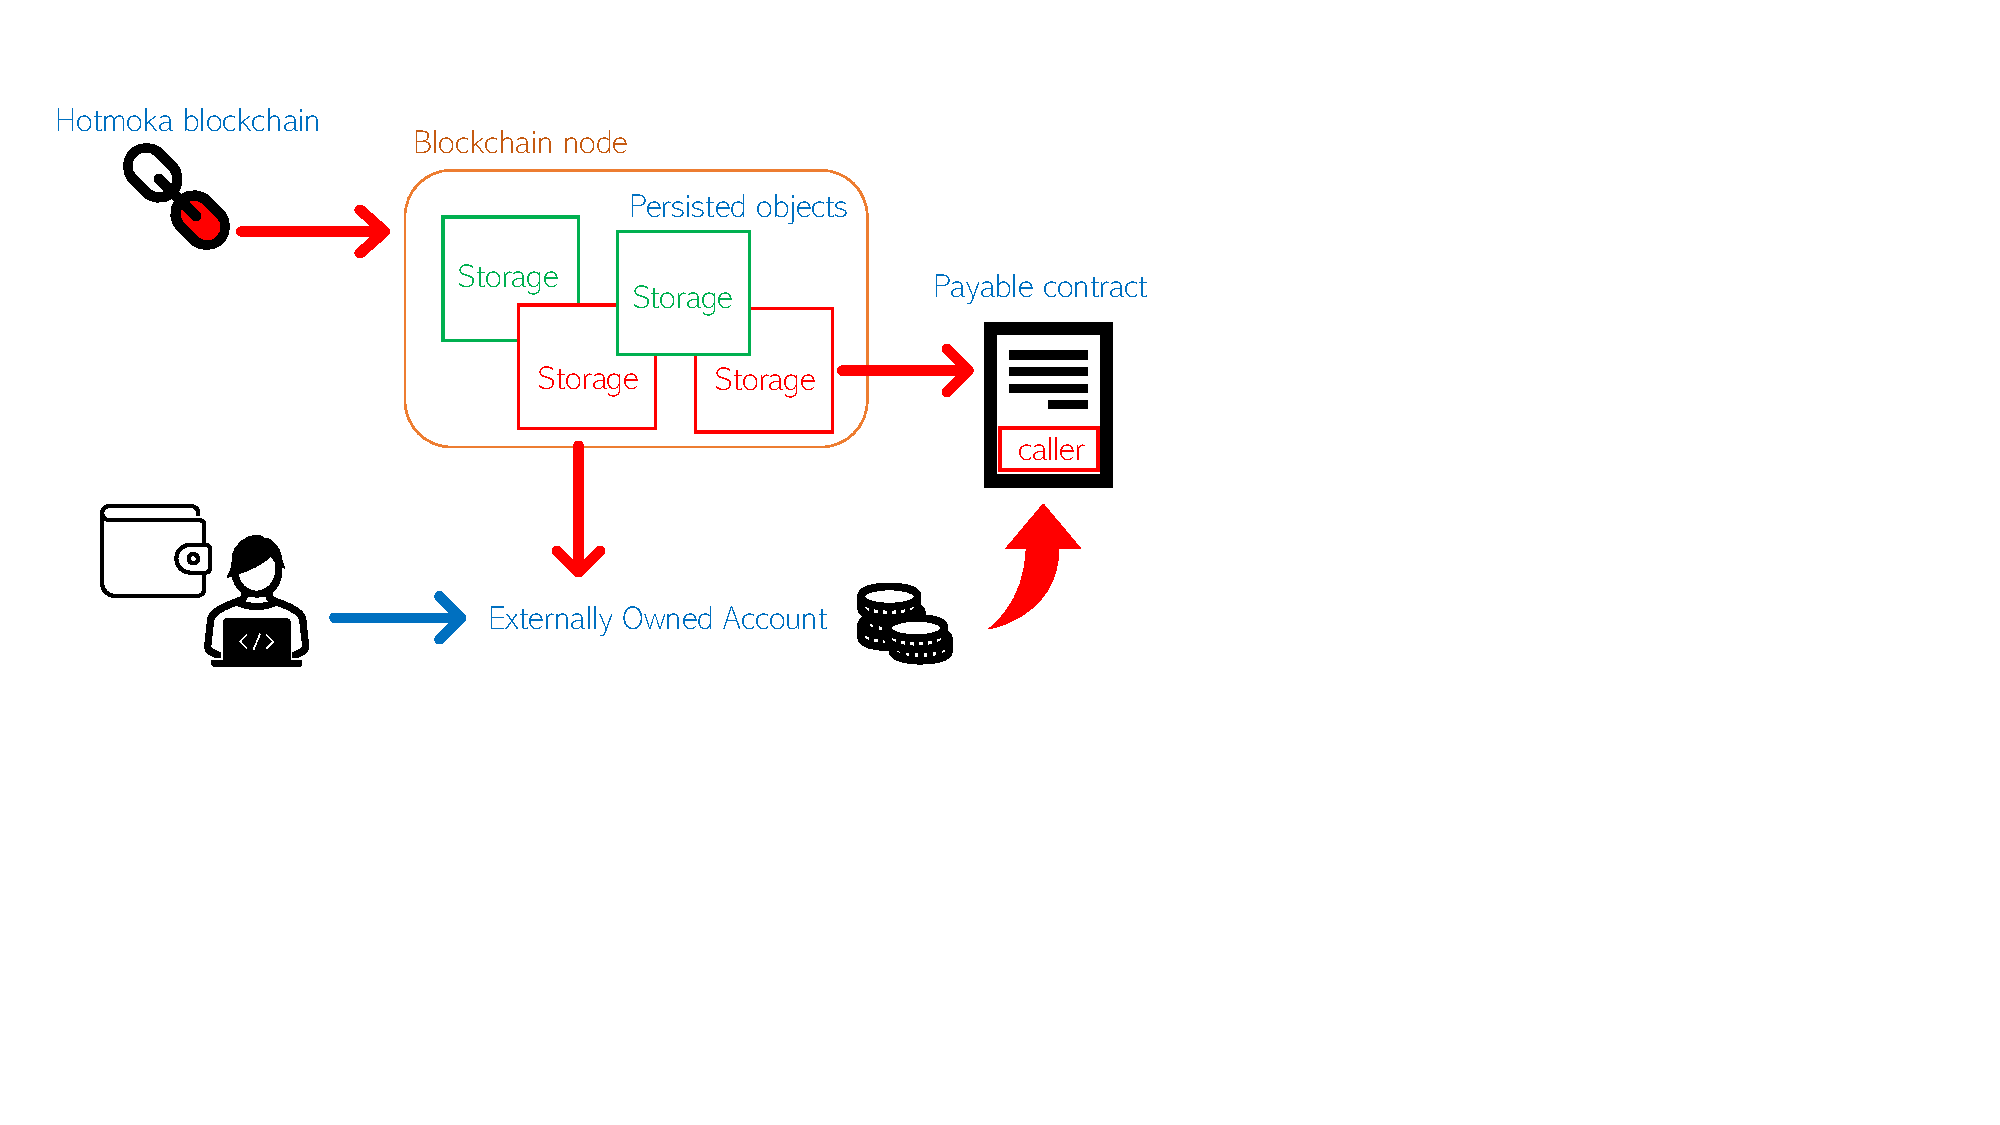
\includegraphics[width=\linewidth]{figures/takamaka_payable_contract}
\caption{Exemplification of the Takamaka persistent objects stored in the blockchain.}
\label{figure.takamaka_payable_contract}
\end{figure}

\begin{figure}[th]
  \begin{center}
    \begin{lstlisting}[language=Takamaka]
public class Validator extends ExternallyOwnedAccount {

  public Validator(String publicKey) {
    super(publicKey);
  }

  public @View String id() {
    return publicKey(); // subclasses may redefine
  }
}

public final class TendermintED25519Validator 
       extends Validator {
  private final String id;

  public TendermintED25519Validator
    (String publicKey) {
    super(publicKey);

    MessageDigest sha256 = 
      MessageDigest.getInstance("SHA-256");
    sha256.update(Base64.getDecoder().
      decode(publicKey()));
    this.id = bytesToHex(sha256.digest()).
      substring(0, 40);
  }

  @Override @View public final String id() {
    return id;
  }
}
    \end{lstlisting}
  \end{center}
  \caption{The account of a validator and its specialization for a Hotmoka blockchain based on Tendermint.}\label{fig:validator}
\end{figure}

Neither the Takamaka language nor the Hotmoka blockchain dictate a specific consensus mechanism.
Both proof of work and proof of stake can be used, for instance. In particular, if proof of stake
is used, then each validator node of the blockchain must specify a
\<io.takamaka.code.governance.Validator> object, that plays the role of the
banking account where the validation rewards of the node get accumulated (see Fig.~\ref{fig:validator}).
It is a special externally owned account, with an extra \<id> method that provides the
identifier of the validator node inside the blockchain network. This identifier depends from the
specific network.
For instance, the subclass
\<io.takamaka.code.governance.tendermint.Tender\-mintED25519Validator>
implements \<id> as for the Tendermint blockchain engine~\cite{Kwon14},
that is,
as the first $40$ hexadecimal digits of the sha256 digest of the Base64-encoded public key
(see its code in Fig.~\ref{fig:validator}).
